\chapter{Evaluation}
\section{Evaluation Methods}
The following section describes the evaluation methods used to generate our benchmark results as well as the advantages and challenges imposed by each method.
\subsection{Performance Benchmark}
\begin{figure}[H]
  \centering
  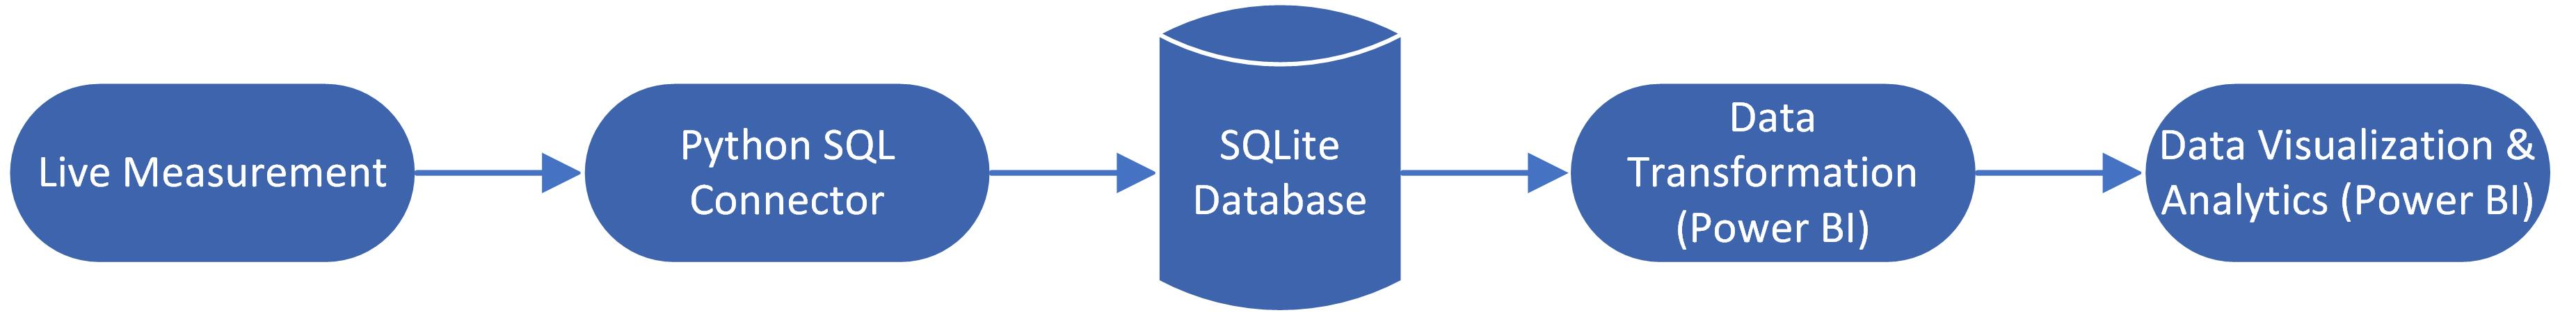
\includegraphics[width=\columnwidth]{media/diagram_reporting.jpg}
  \caption{Analytics Framework}
\end{figure}
The performance of our system was benchmarked on a Raspberry PI Version 3 B+ that was released in March 2018. The PI is powered by a Cortex-A53 quad core processor with 1024 MB of RAM and is equipped with a Raspberry PI camera V2.1.\\
We decided to conduct the performance benchmark with the live feed of the camera instead of using a prerecorded video to replicate our final use case as accurately as possible. In addition to that the decoding of a compressed video stream would have had a significant and measurable impact on the system's overall performance.\\
To produce standardized and comparable benchmark results testing guidelines were used. Every test started with one face at a distance of 0.5 m. After 15 seconds another face was added to measure the impact of tracking multiple faces.
The lighting conditions remained constant for all tested approaches.\\
In addition to the testing performed on the PI all approaches were also benchmarked on a Windows 10 machine with an Intel Core i7-8650U and a \gls{gtx1060} with no processes running in the background.\\
We created a small analytics framework to persist all measurements in a \gls{sqlite} Database. The following data points were captured for every approach: Time of measurement, processing time per frame, method, platform, measurement id and number of faces detected per frame. The \gls{sqlite} database was then connected to \gls{powerbi} to perform further analysis and evaluate the results.
\subsection{Qualitative Benchmark}
The detection quality of the implemented system was evaluated using a mixture of different approaches. To get a first impression of each system's capabilities a subjective test was performed where different factors like lighting and face position (size and tilt) were experimented with. Those experiments were the foundation for a first qualitative assessment.\\
As the approach mentioned above is not quantifiable and does not produce consistent results another method was also used for benchmarking. A clip from "The Late Late Show with James Corden" \cite{latenight} capturing four people in a car in Los Angeles was used to determine the number of faces each approach is able to detect in every frame. An example frame of that clip can be seen in figure \ref{fig:latenight} \cite{jonasbrothers}. The performance metric was then created by calculating the sum of all faces detected over all frames: 
\[
\sum_{Frames}^{} 
\sum_{Faces}^{} 1
\]
In the end both approaches were combined for the final evaluation to achieve maximum flexibility and comparability of the test results.
\begin{figure}[H]
  \centering
  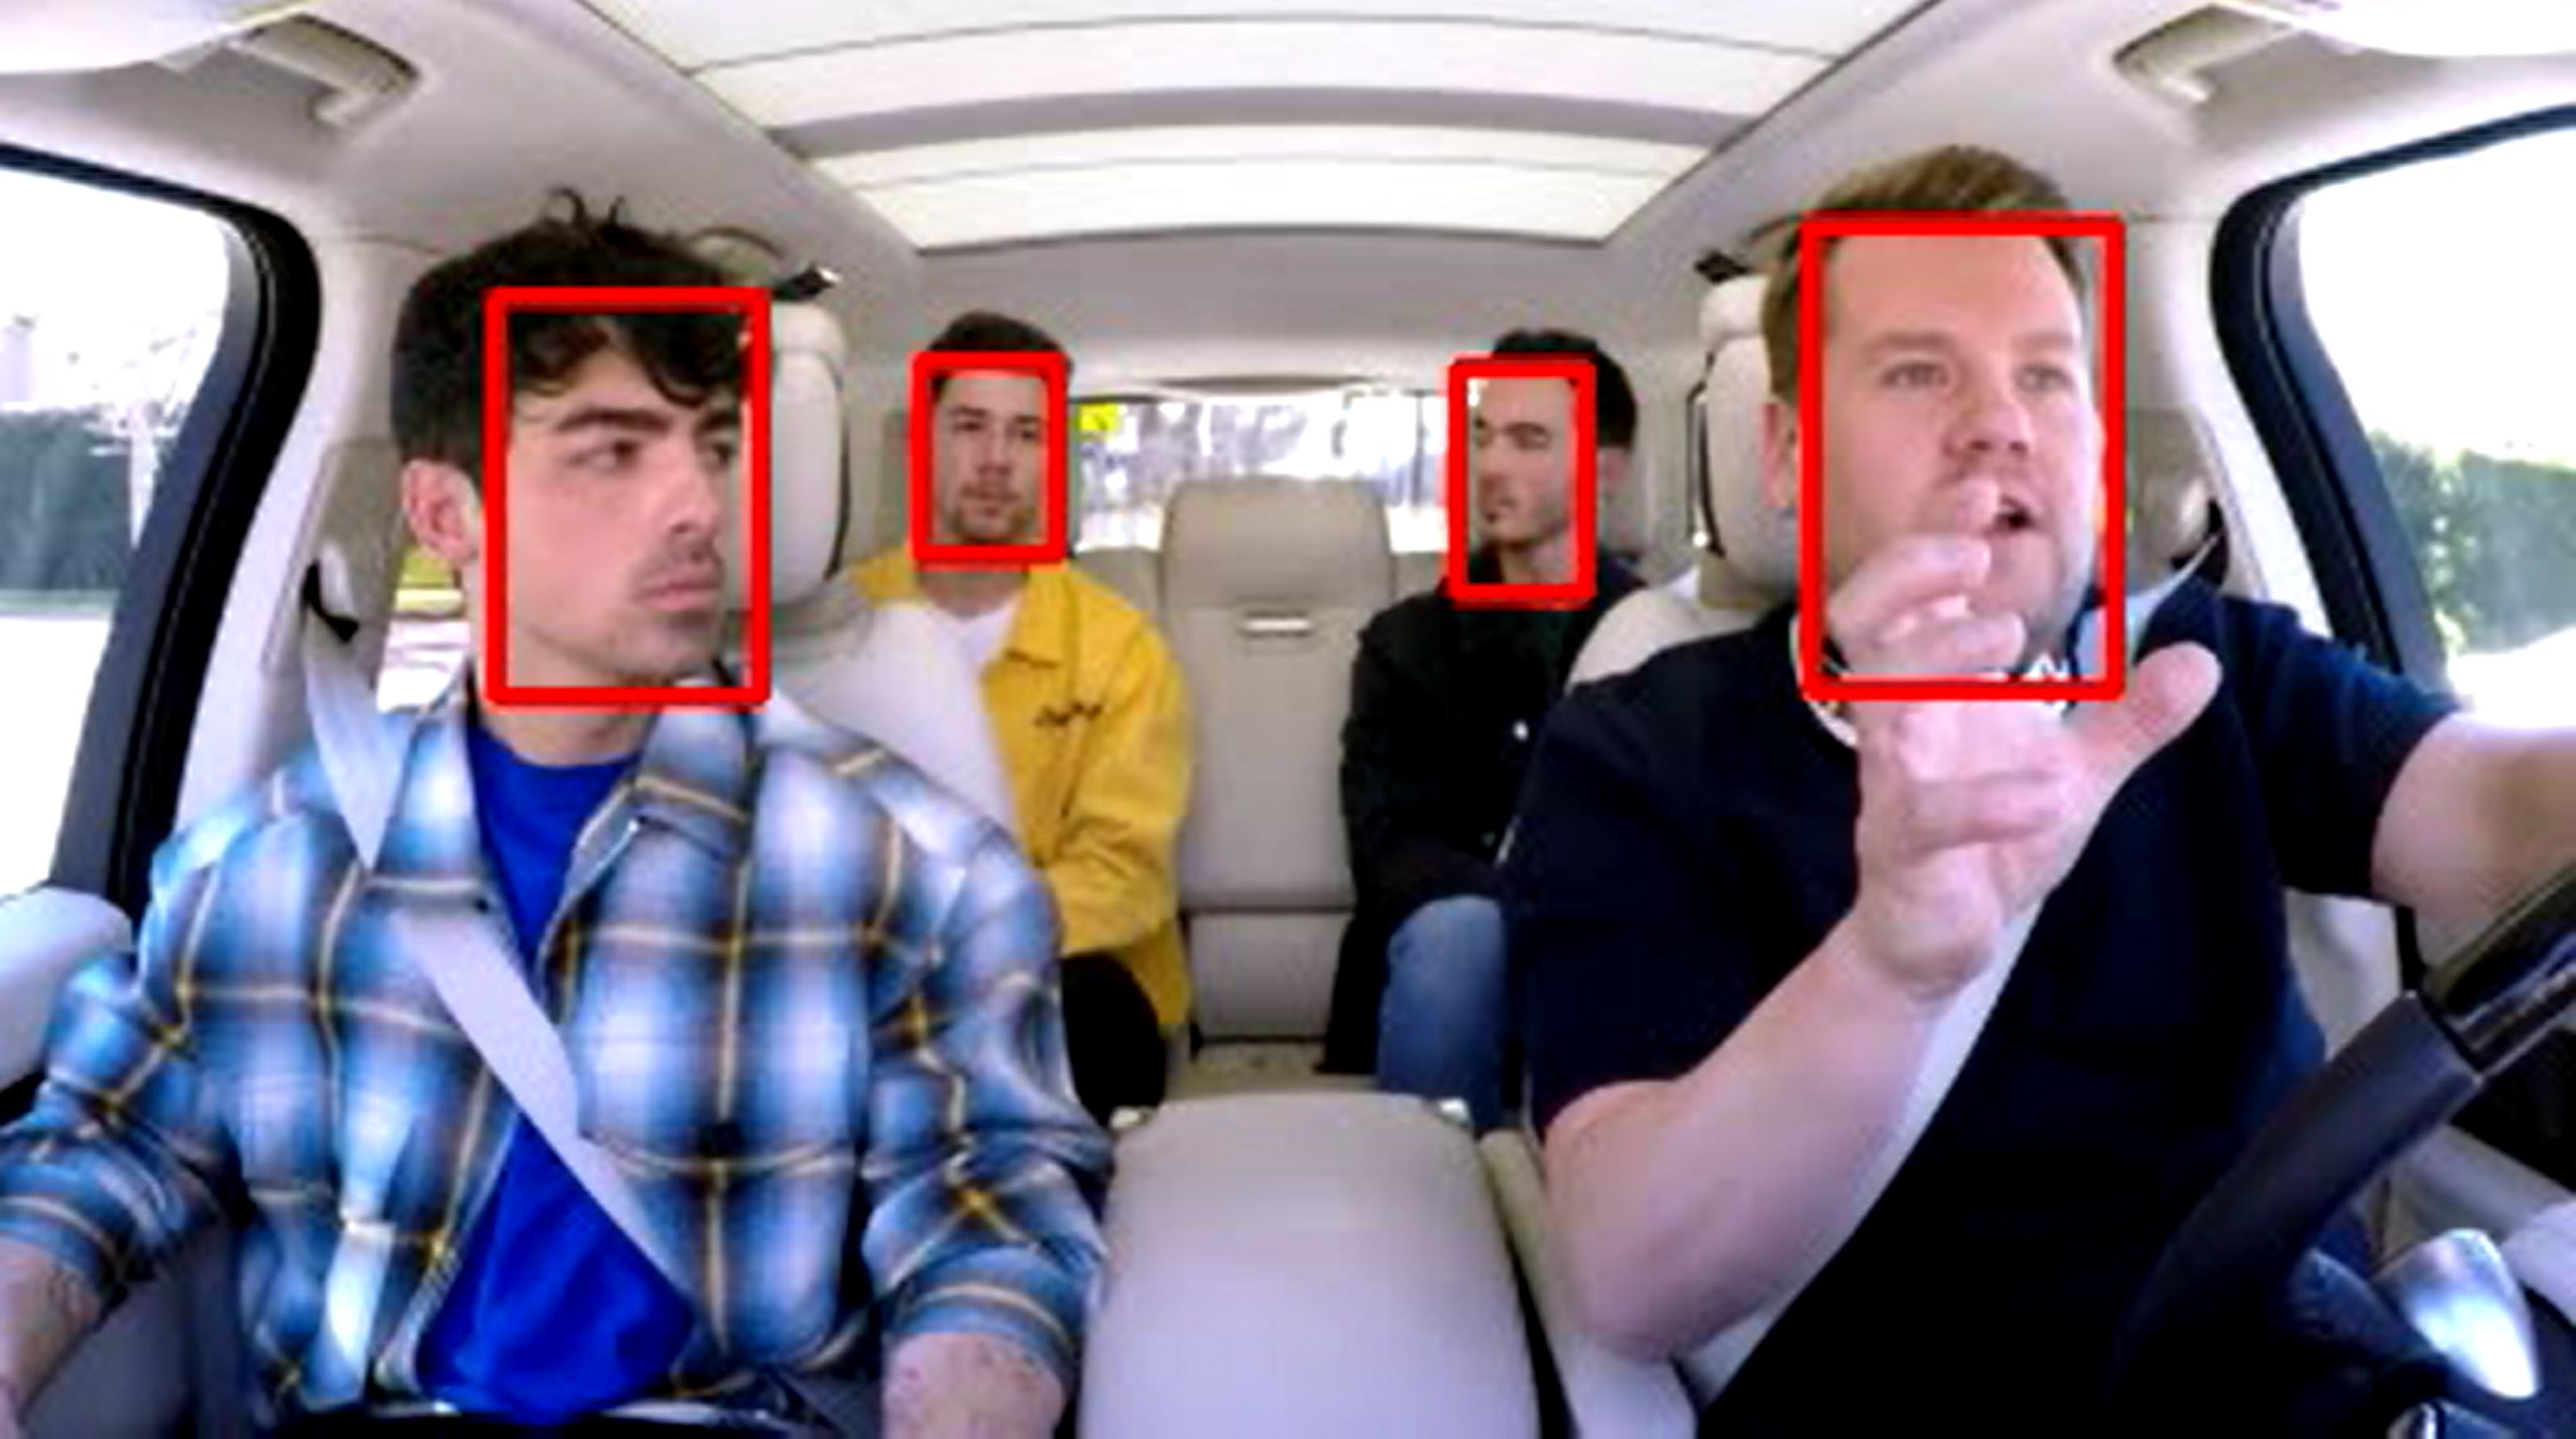
\includegraphics[width=0.8\columnwidth]{media/media_combo.jpg}
  \caption{Jonas Brothers Carpool Karaoke with face detection rectangles}
  \label{fig:latenight}
\end{figure}
\newpage
\section{Evaluation Results}
In the representative benchmarking video our implementation detects 9\% less faces compared to the pretrained \gls{opencv} \gls{cnn}. However, it runs at 10.9 FPS on the Raspberry PI compared to \gls{opencv}'s 0.7 FPS which makes it 16 times faster. The characteristics of our approach and our benchmark results are presented in more detail in the following section. In addition to that advantages and potential issues are highlighted in the data and discussed.\\
\begin{table}[H]
    \resizebox{\textwidth}{!}{
        \begin{tabular}{|l|l|l|l|l|l|}
            \hline
            Platform     & Sample Size & Median Runtime & Average Runtime & $\sigma$   & FPS   \\ \hline
            Windows 10   & 3868        & 0.03           & 0.03            & 0.08 & 32.92 \\ \hline
            Raspberry PI & 1207        & 0.07           & 0.09            & 0.22 & 10.88 \\ \hline
        \end{tabular}
    }
    \caption[Benchmark Results]{Benchmark Results (Definitions in \ref{tab:fdm})}\label{tab:edm}
\end{table}
Figure \ref{fig:edaccuracy} shows the number of faces that our proposed emotion detector was able to detect in the benchmarking video over time. Figure \ref{fig:edfps} plots the frames per second of the implemented system running on a Raspberry Pi over time. There are five areas of relevance which stand out from the rest and will be discussed in the following section.\\
Figure \ref{fig:edaccuracy} A1 highlights a false positive as the system detects 5 people in a car with 4 passengers. False positives are not unusual for networks that were reduced in size and complexity in order to run on an embedded device, however the fact that the false positive remains for a few seconds is special. It is caused by the the object tracker not verifying the validity of a face which leaves the error to remain in the system. We solved this issue by running verification scans every 10 seconds so that new faces added to the frame are detected and errors are removed.\\
The sequence highlighted in figure \ref{fig:edaccuracy} A2 shows another characteristic of our approach. The number of detected faces can remain relatively constant over time and has very little variance. This is because faces - once detected - are tracked very reliably by the KCF object tracker.\\
Figure \ref{fig:edaccuracy} A3 shows the failure mechanism of our approach. As soon as the KCF object tracker loses track of a face (obstacles, occlusion, etc.) the face detector is reinitialized. This should not happen too often in our use case as we assume the number of passengers in the car and their visibility to remain relatively constant. However, this feature will reduce the performance of the system significantly in fast changing environments as can be seen in figure \ref{fig:edfps} A1.\\
Finally figure \ref{fig:edfps} A2 highlights the performance impact of tracking an additional face which is around 2-3 FPS depending on the size of the tracked area.\\
\begin{figure}[H]
\centering
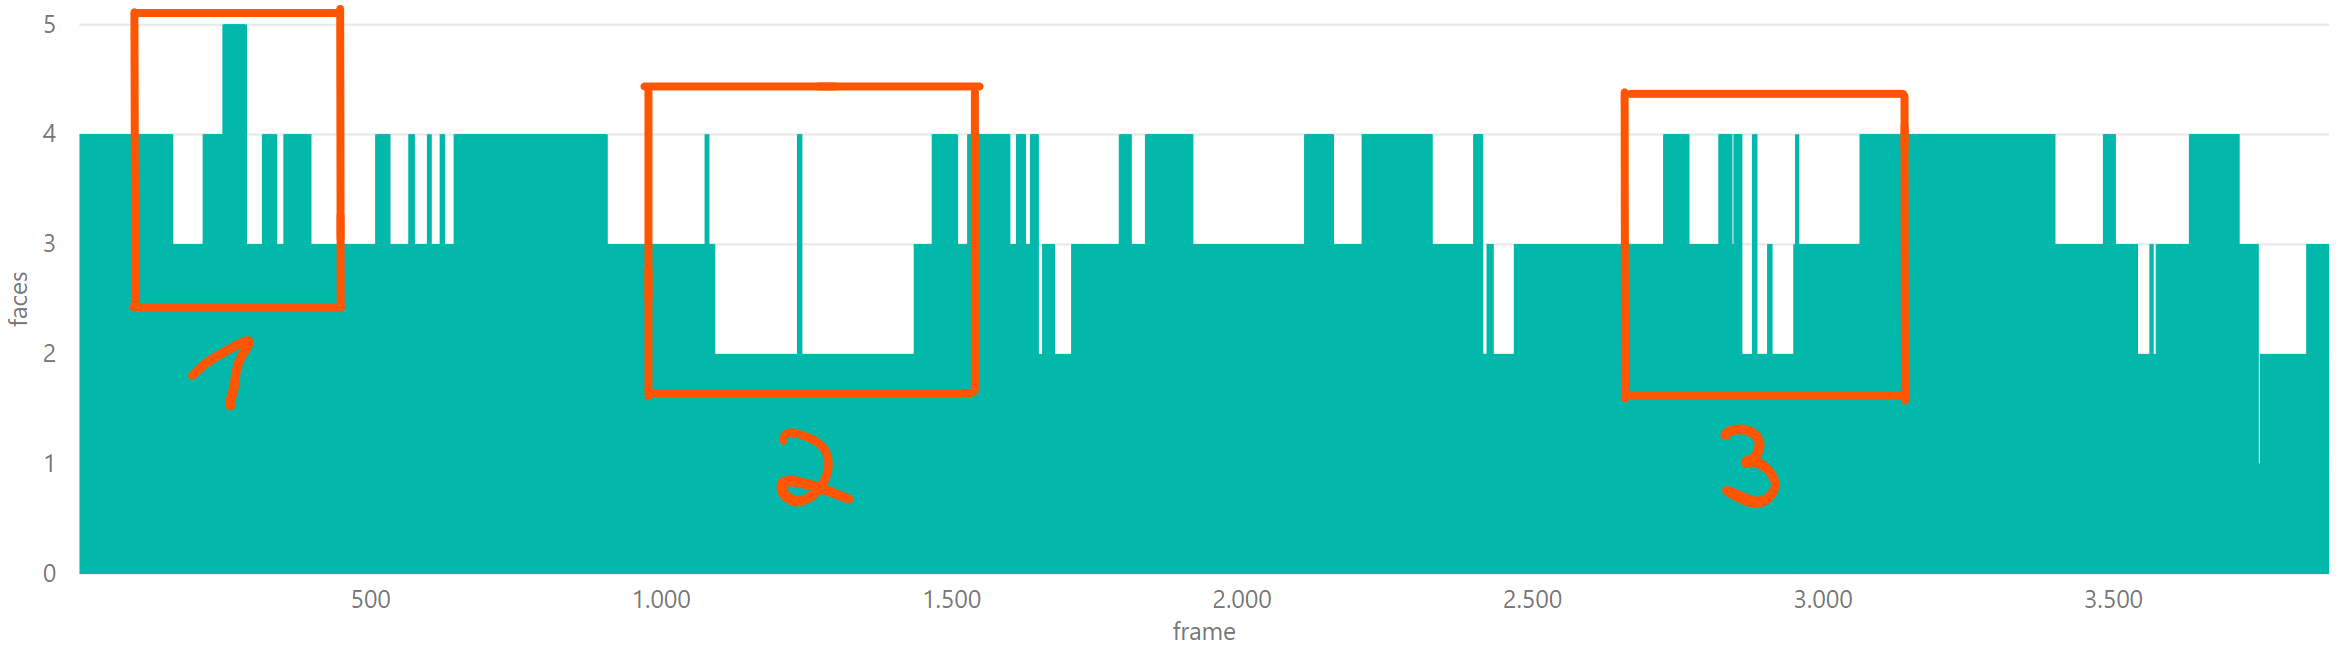
\includegraphics[width=\columnwidth]{media/diagram_ed_accuracy.png}
\caption{Detected faces by the emotion recognition system in the benchmarking video}
\label{fig:edaccuracy}
\end{figure}
\begin{figure}[H]
  \centering
  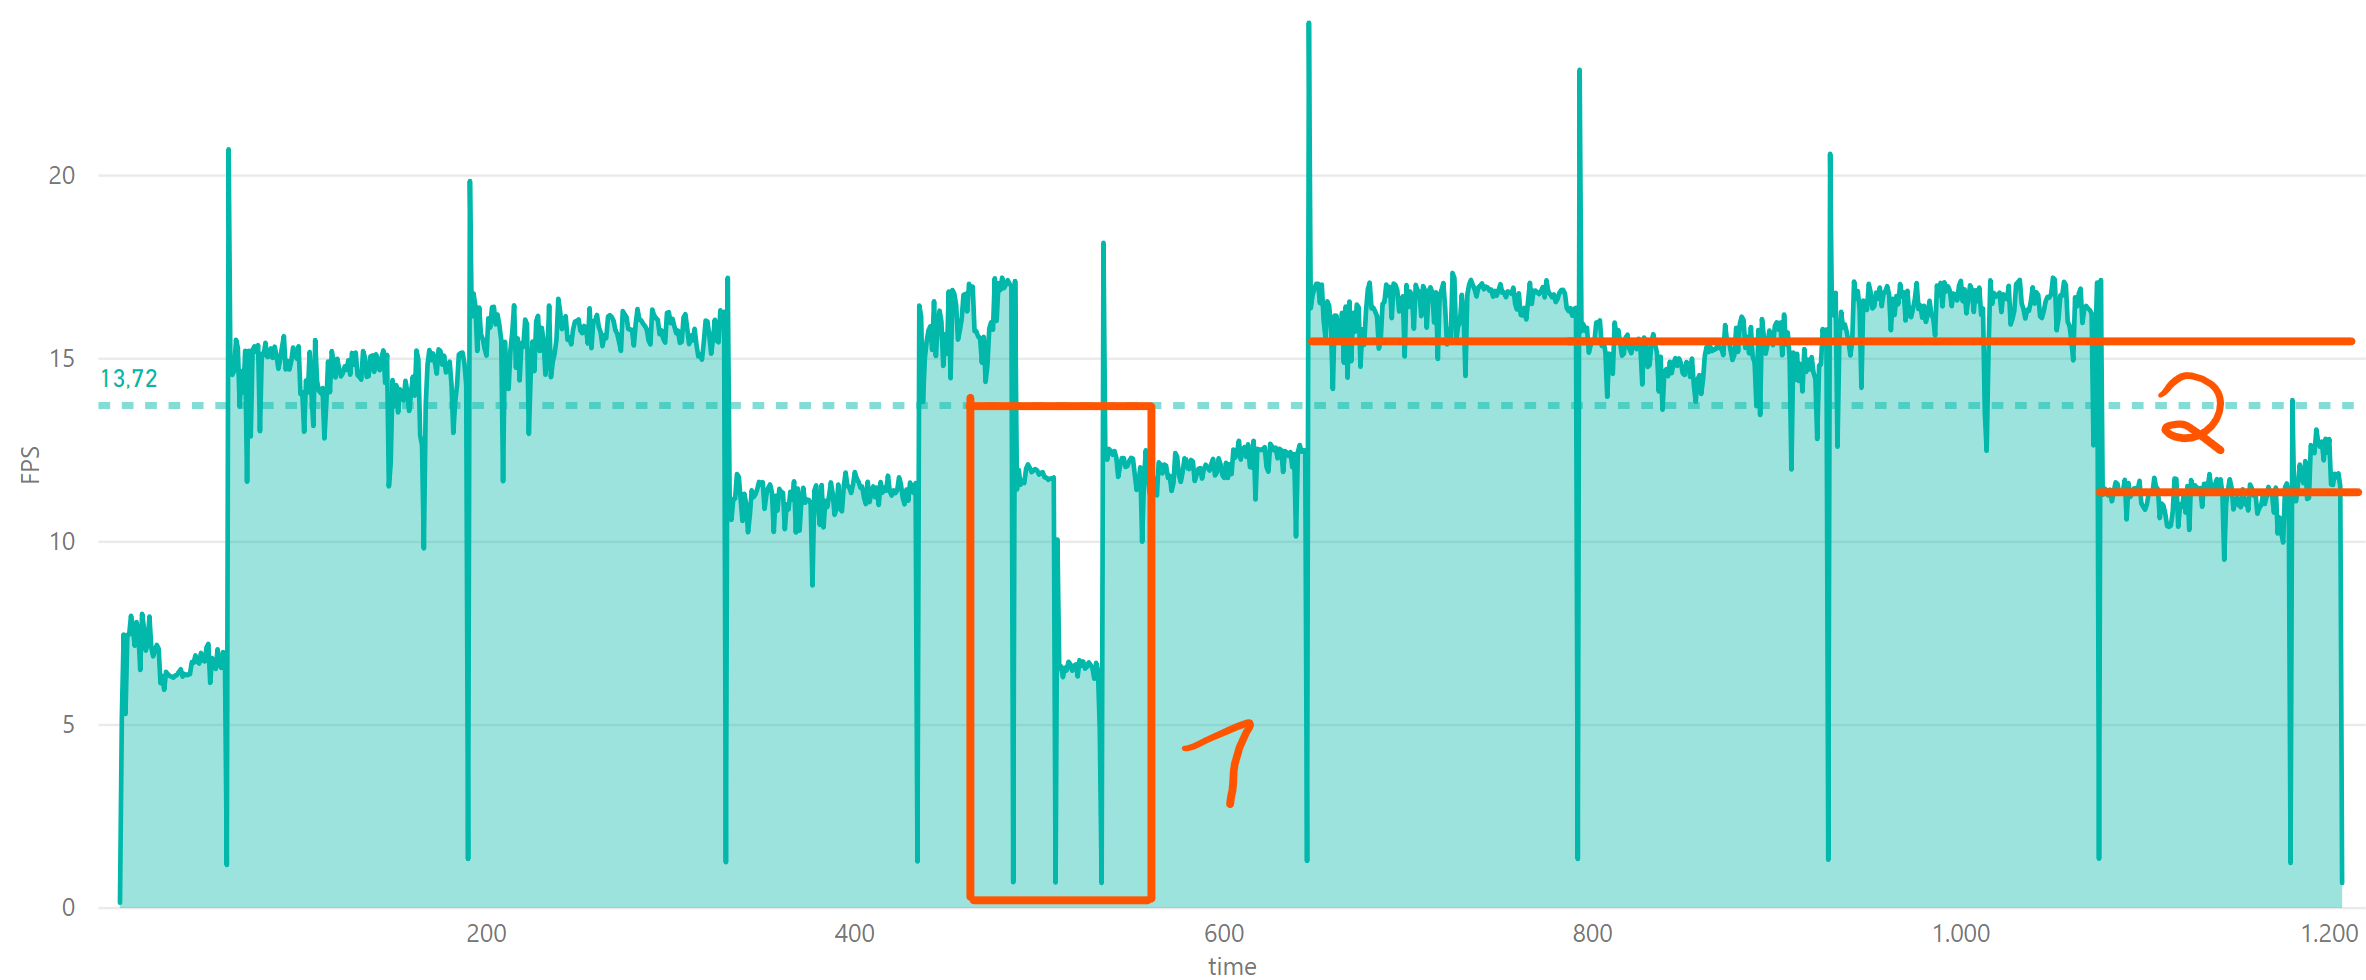
\includegraphics[width=\columnwidth]{media/diagram_ed_FPS_time.png}
  \caption{FPS over time on the Raspberry PI}
  \label{fig:edfps}
\end{figure}